\nonstopmode
\documentclass[12pt]{report}

\title{Multilayer Perceptrons}
\author{}
\date{\today}

\usepackage[
	top=3cm,
	bottom=3cm,
	left=1.5cm,
	right=1.5cm
]{geometry}
\usepackage{amsmath}
\usepackage{amssymb}
\usepackage{amsthm}
\usepackage{amsfonts}
\usepackage{listofitems}
\usepackage{tikz}
\usepackage{pgf}
\usepackage{pgfplots}
\pgfplotsset{compat=1.18}
\usepackage[svgnames, dvipsnames, x11names]{xcolor}
\usepackage[outline]{contour} % glow around text
\usepackage[colorlinks=true, allcolors=black]{hyperref}
\contourlength{1.4pt}

\usepackage[backend=biber, style=numeric]{biblatex}

\addbibresource{./mlp.bib}

% COLORS
\colorlet{myred}{red!80!black}
\colorlet{myblue}{blue!80!black}
\colorlet{mygreen}{green!60!black}
\colorlet{myorange}{orange!70!red!60!black}
\colorlet{mydarkred}{red!30!black}
\colorlet{mydarkblue}{blue!40!black}
\colorlet{mydarkgreen}{green!30!black}
\colorlet{mydarkpurple}{violet!60!black}

\colorlet{mycaptioncol}{myblue!60}

% --------------- FONTS ---------------
% \usepackage{mathptmx}
% \usepackage{newtxtext, newtxmath}
% \usepackage{stix2}
\usepackage{mlmodern} % A better looking version of the default font
\usepackage{roboto}
\usepackage[
	font={small},
	justification=justified,
	labelfont={sf, sc, bf, color=mycaptioncol}
]{caption}
% -------------------------------------

\usetikzlibrary{arrows.meta}

% Reduce spacing for modulo
\renewcommand{\mod}{\;\text{mod}}
% Change the symbol for a QED
\renewcommand{\qedsymbol}{\blacksquare}

% Macro for a set
\newcommand{\set}[1]{\left\{ #1 \right\}}
% Macro for parentheses
\newcommand{\parens}[1]{\left( #1 \right)}
% Macro for angle brackets
\newcommand{\ang}[1]{\left\langle #1 \right\rangle}
% Macro for square brackets
\newcommand{\bracks}[1]{\left[ #1 \right]}

\tikzset{
	declare function={
		lerp(\a,\b,\t) = \a + \t * (\b - \a);
	}
}


% --------- MACROS FOR SYMBOLS ---------

% Define \bbA ... \bbZ for \mathbb
\newcommand{\bbA}{\mathbb{A}}
\newcommand{\bbB}{\mathbb{B}}
\newcommand{\bbC}{\mathbb{C}}
\newcommand{\bbD}{\mathbb{D}}
\newcommand{\bbE}{\mathbb{E}}
\newcommand{\bbF}{\mathbb{F}}
\newcommand{\bbG}{\mathbb{G}}
\newcommand{\bbH}{\mathbb{H}}
\newcommand{\bbI}{\mathbb{I}}
\newcommand{\bbJ}{\mathbb{J}}
\newcommand{\bbK}{\mathbb{K}}
\newcommand{\bbL}{\mathbb{L}}
\newcommand{\bbM}{\mathbb{M}}
\newcommand{\bbN}{\mathbb{N}}
\newcommand{\bbO}{\mathbb{O}}
\newcommand{\bbP}{\mathbb{P}}
\newcommand{\bbQ}{\mathbb{Q}}
\newcommand{\bbR}{\mathbb{R}}
\newcommand{\bbS}{\mathbb{S}}
\newcommand{\bbT}{\mathbb{T}}
\newcommand{\bbU}{\mathbb{U}}
\newcommand{\bbV}{\mathbb{V}}
\newcommand{\bbW}{\mathbb{W}}
\newcommand{\bbX}{\mathbb{X}}
\newcommand{\bbY}{\mathbb{Y}}
\newcommand{\bbZ}{\mathbb{Z}}


% Define \bfA ... \bfZ for \mathbf
\newcommand{\bfA}{\mathbf{A}}
\newcommand{\bfB}{\mathbf{B}}
\newcommand{\bfC}{\mathbf{C}}
\newcommand{\bfD}{\mathbf{D}}
\newcommand{\bfE}{\mathbf{E}}
\newcommand{\bfF}{\mathbf{F}}
\newcommand{\bfG}{\mathbf{G}}
\newcommand{\bfH}{\mathbf{H}}
\newcommand{\bfI}{\mathbf{I}}
\newcommand{\bfJ}{\mathbf{J}}
\newcommand{\bfK}{\mathbf{K}}
\newcommand{\bfL}{\mathbf{L}}
\newcommand{\bfM}{\mathbf{M}}
\newcommand{\bfN}{\mathbf{N}}
\newcommand{\bfO}{\mathbf{O}}
\newcommand{\bfP}{\mathbf{P}}
\newcommand{\bfQ}{\mathbf{Q}}
\newcommand{\bfR}{\mathbf{R}}
\newcommand{\bfS}{\mathbf{S}}
\newcommand{\bfT}{\mathbf{T}}
\newcommand{\bfU}{\mathbf{U}}
\newcommand{\bfV}{\mathbf{V}}
\newcommand{\bfW}{\mathbf{W}}
\newcommand{\bfX}{\mathbf{X}}
\newcommand{\bfY}{\mathbf{Y}}
\newcommand{\bfZ}{\mathbf{Z}}

\newcommand{\bfa}{\mathbf{a}}
\newcommand{\bfb}{\mathbf{b}}
\newcommand{\bfc}{\mathbf{c}}
\newcommand{\bfd}{\mathbf{d}}
\newcommand{\bfe}{\mathbf{e}}
\newcommand{\bff}{\mathbf{f}}
\newcommand{\bfg}{\mathbf{g}}
\newcommand{\bfh}{\mathbf{h}}
\newcommand{\bfi}{\mathbf{i}}
\newcommand{\bfj}{\mathbf{j}}
\newcommand{\bfk}{\mathbf{k}}
\newcommand{\bfl}{\mathbf{l}}
\newcommand{\bfm}{\mathbf{m}}
\newcommand{\bfn}{\mathbf{n}}
\newcommand{\bfo}{\mathbf{o}}
\newcommand{\bfp}{\mathbf{p}}
\newcommand{\bfq}{\mathbf{q}}
\newcommand{\bfr}{\mathbf{r}}
\newcommand{\bfs}{\mathbf{s}}
\newcommand{\bft}{\mathbf{t}}
\newcommand{\bfu}{\mathbf{u}}
\newcommand{\bfv}{\mathbf{v}}
\newcommand{\bfw}{\mathbf{w}}
\newcommand{\bfx}{\mathbf{x}}
\newcommand{\bfy}{\mathbf{y}}
\newcommand{\bfz}{\mathbf{z}}


% Define \calA ... \calZ for \mathcal
\newcommand{\calA}{\mathcal{A}}
\newcommand{\calB}{\mathcal{B}}
\newcommand{\calC}{\mathcal{C}}
\newcommand{\calD}{\mathcal{D}}
\newcommand{\calE}{\mathcal{E}}
\newcommand{\calF}{\mathcal{F}}
\newcommand{\calG}{\mathcal{G}}
\newcommand{\calH}{\mathcal{H}}
\newcommand{\calI}{\mathcal{I}}
\newcommand{\calJ}{\mathcal{J}}
\newcommand{\calK}{\mathcal{K}}
\newcommand{\calL}{\mathcal{L}}
\newcommand{\calM}{\mathcal{M}}
\newcommand{\calN}{\mathcal{N}}
\newcommand{\calO}{\mathcal{O}}
\newcommand{\calP}{\mathcal{P}}
\newcommand{\calQ}{\mathcal{Q}}
\newcommand{\calR}{\mathcal{R}}
\newcommand{\calS}{\mathcal{S}}
\newcommand{\calT}{\mathcal{T}}
\newcommand{\calU}{\mathcal{U}}
\newcommand{\calV}{\mathcal{V}}
\newcommand{\calW}{\mathcal{W}}
\newcommand{\calX}{\mathcal{X}}
\newcommand{\calY}{\mathcal{Y}}
\newcommand{\calZ}{\mathcal{Z}}

% --------------------------------------

\newcommand{\reffig}[1]{Figure~\ref{#1}}

% Math Operators
\DeclareMathOperator{\softmax}{softmax}
\DeclareMathOperator{\ReLU}{ReLU}
\DeclareMathOperator{\SiLU}{SiLU}
\DeclareMathOperator{\GELU}{GELU}
\DeclareMathOperator{\erf}{erf}

% Macro for gradient
\newcommand{\grad}{\nabla}

\newcommand{\dd}[2]{\frac{d #1}{d #2}}
\newcommand{\ddn}[3]{\frac{d^{#3} #1}{{d#2}^{#3}}}
\newcommand{\DD}[2]{\frac{\partial #1}{\partial #2}}
% no completion in denominator in order to support mixed partials
\newcommand{\DDN}[3]{\frac{\partial^{#3} #1}{#2}}
\newcommand{\dps}[1]{{\displaystyle #1}}

\newcommand{\veps}{\varepsilon}

\newcommand{\bracetext}[2]{\underset{#2}{\underbrace{#1}}}

% =============================================
% NEURAL NETWORK DRAWING LOGIC 
% https://tikz.net/neural_networks/
% =============================================

% STYLES
\tikzset{
  >=latex, % for default LaTeX arrow head
  node/.style={thick,circle,draw=myblue,minimum size=22,inner sep=0.5,outer sep=0.6},
  node in/.style={node,green!20!black,draw=mygreen!30!black,fill=mygreen!25},
  node hidden/.style={node,blue!20!black,draw=myblue!30!black,fill=myblue!20},
  node convol/.style={node,orange!20!black,draw=myorange!30!black,fill=myorange!20},
  node out/.style={node,red!20!black,draw=myred!30!black,fill=myred!20},
  connect/.style={thick,mydarkblue}, %,line cap=round
  connect arrow/.style={-{Latex[length=4,width=3.5]},thick,mydarkblue,shorten <=0.5,shorten >=1},
  node 1/.style={node in}, % node styles, numbered for easy mapping with \nstyle
  node 2/.style={node hidden},
  node 3/.style={node out}
}
\def\nstyle{int(\lay<\Nnodlen?min(2,\lay):3)} % map layer number onto 1, 2, or 3

\pgfmathsetseed{12345}

% =============================================================
% AXES STYLE
% =============================================================

\tikzset{
	point/.style = {
		draw,
		circle,
		fill,
		inner sep = 0pt,
		minimum size = 4pt,
	},
}

\pgfplotsset{
	plane/.style={
		axis equal image,
		axis lines = middle,
		axis line style = {->},
		xlabel style = {at={(axis description cs: 1.02, 0)}, anchor = west},
		ylabel style = {at={(axis description cs: 0, 1.02)}, anchor = south},
		grid = both,
		minor tick num = 5, 
		major grid style = {thin, black!50},
		minor grid style = {very thin, black!30}
	}
}

% Arg1: General extra args for axis
% Arg2: Major grid line color + extra args
% Arg3: Minor grid line color + extra args
\NewDocumentEnvironment{plane}{O{}O{black!50}O{black!30}}{
	\begin{axis}[
		plane,
		major grid style={thin, #2},
		minor grid style={very thin, #3},
		#1
	]
}{
	\end{axis}
}

\begin{document}

\maketitle

\tableofcontents

\chapter{The Basics of Multilayer Perceptrons}

A \textbf{multilayer perceptron} (otherwise known as a \textit{neural network}) is a set of nodes called \textbf{neurons}, each containing an activation -- a number (usually) between 0 and 1 -- which designates how active that specific neuron is.

This is loosely analogous to how our brains work, where each of our neurons can fire to send an electrical signal which, somewhere down the chain, might move our arm or let us perceive the smell of some food.

The image people usually associate with neural networks is the following:

\begin{figure}[ht]
	\centering
	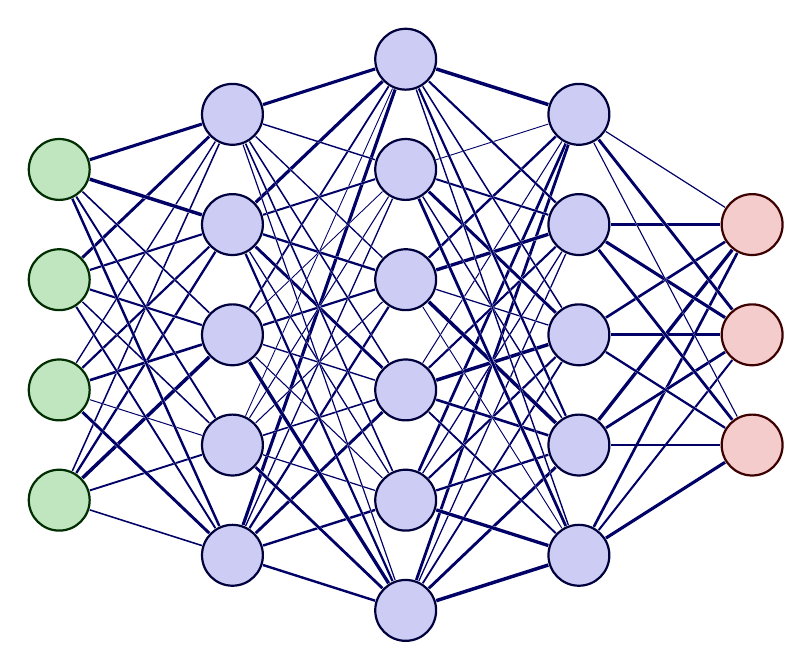
\begin{tikzpicture}[x=2.2cm,y=1.4cm]
		\readlist\Nnod{4,5,6,5,3} % array of number of nodes per layer

		% \message{^^J  Layer}
		\foreachitem \N \in \Nnod{
			\def\lay{\Ncnt} % alias of index of current layer
			\pgfmathsetmacro\prev{int(\Ncnt-1)} % number of previous layer
			% \message{\lay,}
			\foreach \i [evaluate={\y=\N/2-\i; \x=\lay; \n=\nstyle;}] in {1,...,\N}{ % loop over nodes
				  
				% NODES
				\node[node \n] (N\lay-\i) at (\x,\y) {};

				% CONNECTIONS
				\ifnum\lay>1 % connect to previous layer
					\foreach \j in {1,...,\Nnod[\prev]}{ % loop over nodes in previous layer
						\pgfmathsetmacro{\w}{0.3 + rnd}
						\draw[connect,white,line width=1.2*\w] (N\prev-\j) -- (N\lay-\i);
						\draw[connect, line width=\w] (N\prev-\j) -- (N\lay-\i);
						%\draw[connect] (N\prev-\j.0) -- (N\lay-\i.180); % connect to left
					}
				\fi % else: nothing to connect first layer
			}
		}

		% \node[above=5,align=center,mygreen!60!black] at (N1-1.90) {input\\[-0.2em]layer};
		% \node[above=2,align=center,myblue!60!black] at (N3-1.90) {hidden layers};
		% \node[above=10,align=center,myred!60!black] at (N\Nnodlen-1.90) {output\\[-0.2em]layer};
	\end{tikzpicture}
	\caption{A simple neural network.}
	\label{fig:neural-net-simple}
\end{figure}

\reffig{fig:neural-net-simple} shows the structure of a neural network. At its core, a neural network has an \textbf{input layer} (colored in green), analogous to some sensory input such as our eyes capturing the light around us, an \textbf{output layer} (colored in red), analogous to the output of our vision, which is a colored image of our environment, and then some ``hidden layers,'' which are basically the meat of the network and encode everything about how the inputs and corresponding outputs are related to one another.

\vspace{12pt}

The actual math behind these networks is surprisingly simple. We'll focus on a single connection for now:

\begin{figure}[ht]
	\centering
	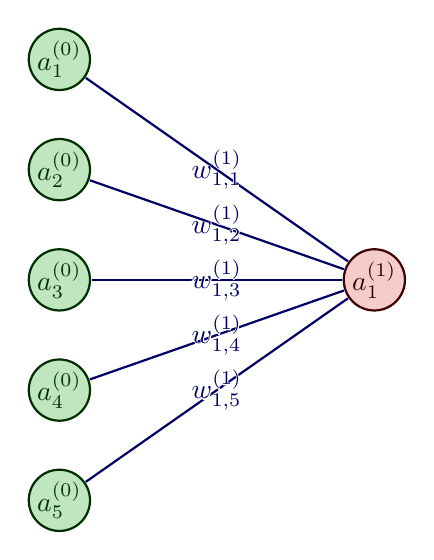
\begin{tikzpicture}[y=1.4cm]
		\def\NI{5}
		\node[node 3] (second) at (2, 0) {$a_1^{(1)}$};
		\foreach \i [evaluate={\y=(\NI + 1) / 2 - \i; \index = int(\i)}] in {1,...,\NI} {
			\node[node 1] (NI-\i) at (-2, \y) {$a_{\index}^{(0)}$};
			\draw[connect] (NI-\i) -- (second) node[midway] {\contour{white}{$w_{1,\index}^{(1)}$}};
		}
	\end{tikzpicture}
	\caption{The activation of two neurons and the weight between them.}
	\label{fig:neuron-activation-example}
\end{figure}

Let's decypher these symbols one-by-one:
\begin{itemize}
	\item ${\color{mydarkgreen} a_n^{(0)}}$: The activations of the neurons within the first layer.
	\item ${\color{mydarkblue} w_{1,n}^{(1)}}$: The \textbf{weights} of each of the connections. Essentially, this encodes how strongly connected the neurons are (so how much they influence each-other).
	\item ${\color{mydarkred} a_1^{(1)}}$: The output activation.
\end{itemize}

In order to determine the output activation $a_1^{(1)}$ from the input activations $a_i^{(0)}$, we simply take a weighted sum whose weights are the coefficients $w_{1,i}^{(1)}$; that is,
\[
	{\color{mydarkred} a_1^{(1)}} = {\color{mydarkblue} w_{1,1}^{(1)}}{\color{mydarkgreen} a_1^{(0)}} + {\color{mydarkblue} w_{1,2}^{(1)}}{\color{mydarkgreen} a_2^{(0)}} + \cdots + {\color{mydarkblue} w_{1,5}^{(1)}}{\color{mydarkgreen} a_5^{(0)}}
\]

Usually we also add in what's called a \textbf{bias} term, which is just a value that we add to this sum. We can interpret the bias as the ``sensitivity'' of the neuron. That means that the whole expression in the general case (so, for $n$ neurons in the input layer) is
\[
	{\color{mydarkred} a_1^{(1)}} = {\color{mydarkpurple}b_1^{(1)}} + \sum_{i=1}^{n}{\color{mydarkblue} w_{1,i}^{(1)}}{\color{mydarkgreen} a_i^{(0)}}
\]

There's only one issue: Remember we said that the activations must be between 0 and 1, but with a weighted sum like this, we can essentially get any number. What we need now is some kind of way to squish this value into the range $[0,1]$. The most common function for this purpose is the \textbf{sigmoid} function:
\[
	{\color{mydarkred}\sigma({\color{mydarkblue}x})} = \frac{1}{1 + e^{-{\color{mydarkblue}x}}}
\]

The graph of this function is shown below:

\begin{figure}[ht]
	\centering
	\begin{tikzpicture}
		\begin{plane}[
			tick label style = {font = \small},
			xmin = -4,
			xmax = 4,
			ymin = -3,
			ymax = 3
		]
			\addplot[mydarkblue, smooth, ultra thick] {1 / (1 + exp(-x))};
		\end{plane}
	\end{tikzpicture}
	\caption{The graph of $\sigma(x)$.}
	\label{fig:sigmoid-graph}
\end{figure}

\newpage

From \reffig{fig:sigmoid-graph}, we can see how the function approaches 0 when $x$ is negative, and approaches 1 when $x$ is positive. This is exactly what we needed! Putting all of this together, we have the following expression for ${\color{mydarkred}a_1^{(1)}}$:
\[
	{\color{mydarkred}a_1^{(1)}} = {\color{mydarkred}\sigma}{\color{mydarkred}\Bigg(}{\color{mydarkpurple}b_1^{(1)}}{\color{black} + \sum_{i=1}^{n}}{\color{mydarkblue}w_{1,i}^{(1)}}{\color{mydarkgreen}a_i^{(0)}}{\color{mydarkred}\Bigg)}
\]

Remember, this is just for the activation of a \textit{single} neuron, so for a whole layer, we need to do this many times. There is a way we can simplify this, but we'll need to consider the more general case in order to do so.

\begin{figure}[ht]
	\centering
	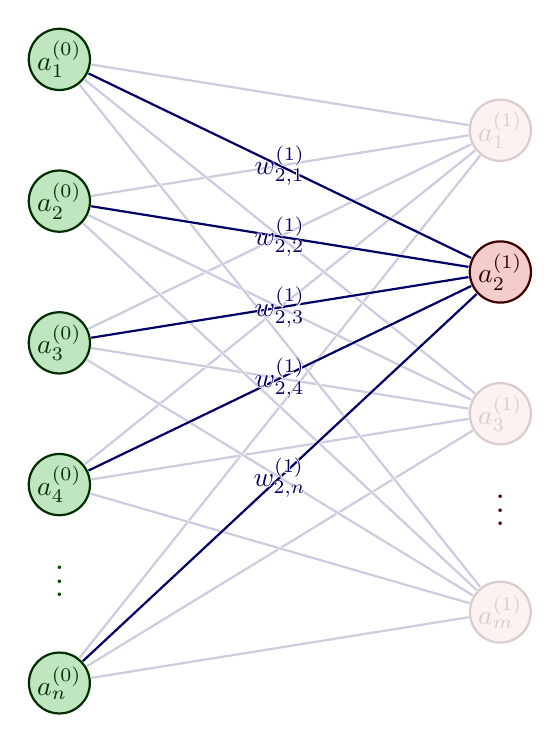
\begin{tikzpicture}[x=1.4cm, y = 1.8cm]
		\def\NI{5}
		\def\NO{4}
		\def\NodeFocused{2}
		\def\yshift{0.4}

		% Input Layer
		\foreach \i [evaluate={\c=int(\i==\NI); \y=\NI / 2 - \i - \c*\yshift; \index=(\i < \NI ? int(\i) : "n");}] in {1,...,\NI}{
			\node[node in] (NI-\i) at (-2,\y) {$a_{\index}^{(0)}$};
		}

		\foreach \i [evaluate={\c=int(\i==\NO); \y=\NO / 2 - \i - \c * \yshift; \indexout = (\i < \NO ? int(\i) : "m");}] in {1,...,\NO}{
			\ifnum\i=\NodeFocused
				% skip for now
			\else
				\node[node, color=mydarkred!20, fill=myred!5] (NO-\i) at (2,\y) {$a_{\indexout}^{(1)}$};
				\foreach \j [evaluate={\indexin=int(\j);}] in {1,...,\NI}{
					\draw[connect, white, line width = 1.2] (NI-\j) -- (NO-\i);
					\draw[connect, mydarkblue!20] (NI-\j) -- (NO-\i);
				}
			\fi
		}

		\pgfmathsetmacro\yfocused{\NO/2-\NodeFocused-int(\NodeFocused==\NO) * \yshift}
		\pgfmathsetmacro\indexout{(\NodeFocused < \NO ? int(\NodeFocused) : "m")}
		
		% Draw the focused node after everything else
		\node[node out] (NO-\NodeFocused) at (2,\yfocused) {$a_{\indexout}^{(1)}$};

		\foreach \j [evaluate={\indexin=(\j < \NI ? int(\j) : "n");}] in {1,...,\NI}{
			\draw[connect, white, line width = 1.2] (NI-\j) -- (NO-\NodeFocused);
			\draw[connect] (NI-\j) -- (NO-\NodeFocused) node[midway] {\contour{white}{$w_{\indexout,\indexin}^{(1)}$}};
		}

		\path[color=mydarkgreen] (NI-\NI) --++ (0,0.95+\yshift) node[midway,scale=1.2] {$\vdots$};
	  \path[color=mydarkred] (NO-\NO) --++ (0,0.95+\yshift) node[midway,scale=1.2] {$\vdots$};
	\end{tikzpicture}
	\caption{The general case of the connections between two layers.}
	\label{fig:general-connection-case}
\end{figure}

The key insight here is that we can simplify this process immensely with the tools of linear algebra. In particular, we can group all the activations in the first layer (layer 0) into a column vector:
\[
	{\color{mydarkgreen} \bfa^{(0)}} = {\color{mydarkgreen}\begin{bmatrix}
			a_1^{(0)}\\
			a_2^{(0)}\\
			\vdots\\
			a_n^{(0)}
	\end{bmatrix}}
\]

\noindent
We can do the same thing for the output activations:
\[
	{\color{mydarkred} \bfa^{(1)}} = {\color{mydarkred}\begin{bmatrix}
			a_1^{(1)}\\
			a_2^{(1)}\\
			\vdots\\
			a_m^{(1)}
		\end{bmatrix}}
\]

\noindent
Similarly, we can group the biases up into a vector as well:
\[
	{\color{mydarkpurple} \bfb^{(1)}} = {\color{mydarkpurple}\begin{bmatrix}
			b_1^{(1)}\\
			b_2^{(1)}\\
			\vdots\\
			b_m^{(1)}
		\end{bmatrix}}
\]

\noindent
Finally, the weights simply become a matrix which we multiply with ${\color{mydarkgreen}\bfa^{(0)}}$:

\[
	{\color{mydarkblue} \bfW^{(1)}} = {\color{mydarkblue}\begin{bmatrix}
			w_{1,1}^{(1)} & w_{1,2}^{(1)} & w_{1,3}^{(1)} & \cdots & w_{1,n}^{(1)}\\
			w_{2,1}^{(1)} & w_{2,2}^{(1)} & w_{2,3}^{(1)} & \cdots & w_{2,n}^{(1)}\\
			w_{3,1}^{(1)} & w_{3,2}^{(1)} & w_{3,3}^{(1)} & \cdots & w_{3,n}^{(1)}\\
			\vdots  & \vdots & \vdots  & \ddots & \vdots \\
			w_{m,1}^{(1)} & w_{m,2}^{(1)} & w_{m,3}^{(1)} & \cdots & w_{m,n}^{(1)}
		\end{bmatrix}}
\]

\noindent
Now, if we imply that the function $\sigma(x)$ applies component-wise to vectors and matrices, we get the following incredibly neat formula for the activations in layer $L + 1$ given those in layer $L$:
\[
	{\color{mydarkred}\bfa^{(L+1)}} = {\color{mydarkred}\sigma}{\color{mydarkred}\big(}{\color{mydarkpurple}\bfb^{(L+1)}} + {\color{mydarkblue}\bfW^{(L+1)}}{\color{mydarkgreen}\bfa^{(L)}}{\color{mydarkred}\big)}
\]

\newpage

\section*{Other Activation Functions}

The sigmoid is not the only function we can use to remap our values. In fact, there are infinitely many functions we can use. Another common choice is the $\tanh$ function (which remaps values between $-1$ and 1). Beyond that, we sometimes don't want to remap between finite values at all. This is why other (arguably more common) activation functions include the $\ReLU$, $\SiLU$, and, more recently, $\GELU$ functions.

\begin{figure}[ht]
	\centering
	\begin{tikzpicture}[
		declare function={
			sigmoid(\x) = 1 / (1 + exp(-\x));
			relu(\x) = max(\x, 0);
			silu(\x) = \x * sigmoid(\x);
			gelu(\x) = 0.5 * \x * (1 + tanh(sqrt(2 / pi) * (\x + 0.044715 * \x^3)));
		},
		scale=1.25
	]
		\begin{plane}[
			xmin = -3,
			xmax = 3,
			ymin = -3,
			ymax = 3,
			legend style = {font=\scriptsize},
			legend cell align=left,
			legend pos = north west,
			tick label style = {font = \small},
		]
			\addplot[very thick, smooth, black] {tanh(x)};
			\addlegendentry{$\tanh(x)$}
			\addplot[very thick, smooth, LimeGreen] {silu(x)};
			\addlegendentry{$\SiLU(x)$}
			\addplot[very thick, smooth, TealBlue] {gelu(x)};
			\addlegendentry{$\GELU(x)$}
			\addplot[very thick, smooth, samples=200, OrangeRed] {relu(x)};
			\addlegendentry{$\ReLU(x)$}
		\end{plane}
	\end{tikzpicture}
	\caption{The graphs of the different activation functions.}
	\label{fig:activation-functions}
\end{figure}

$\ReLU$ is very common because it's very strict for model behavior; the activation simply gets clamped to zero if it's negative. The expressions for these functions are the following:
\begin{align*}
	\ReLU(x) &= \max(x, 0)\\
	\SiLU(x) &= x \sigma(x)\\
	\GELU(x) &\approx 0.5x\parens{1 + \tanh\parens{\sqrt{\frac{2}{\pi}}\parens{x + 0.044715x^3}}}\text{\cite{hendrycks2023gelu}}
\end{align*}

The expression for $\GELU$ is simply an approximation because it is actually derived from the cumulative distribution function of the normal distribution, which has no elementary form. In fact, the \textit{true} expression defining $\GELU(x)$ is 
\[
	\GELU(x) = x\Phi(x) = x\frac{1}{2}\bracks{1 + \erf\parens{\frac{x}{\sqrt{2}}}},
\]
where 
\[
	\erf(x) = \int_0^x e^{-s^2}ds
\]
is the error function.

\chapter{Backpropagation: How Neural Networks Learn}

This chapter is all about one of the most important algorithms in deep learning: backpropagation. Essentially, this is how a neural network is able to ``learn'' from its training data. At a high level, the way it works is that it takes the prediction of the model, compares it with the expected output, and uses how far they are from each other to adjust the weights and biases of the model.

\section{Cost or Loss Functions}

At the core of backpropagation is the idea of a \textbf{cost function} or \textbf{loss function}. This is the function which, given the model's prediction and the target value, returns some number indicating how badly the model performed. Then, once we have this mysterious function, backpropagation comes down to a simple optimization problem -- we'll want to minimize whatever this function is.

There are tons of loss functions out there, but the two most common ones are MSE (mean squared error) loss and cross-entropy loss. MSE loss is good for general purpose models, whilst cross-entropy is specifically designed for models whose objective is some sort of classification (such as for the classic MNIST model).

\vspace{12pt}

The definition for MSE loss is quite straightforward. Given a model output $\bfy$ and a target output $\hat{\bfy}$, the MSE loss is simply the average of their squared difference. Mathematically, assuming that $\bfy,\hat{\bfy}\in\bbR^n$,
\[
	\text{MSE} = \frac{1}{n} \sum_{i=1}^n (y_i - \hat{y}_i)^2 
\]

The main reason this is such a popular choice is that it's incredibly easy to differentiate, since it's just a power. It's also very intuitive: the amount the model deviates from the target is just the average difference between its output and the target, and we square it so that the values are all positive while keeping the function differentiable. 

\vspace{12pt}

Cross-entropy, on the other hand, has a few nuances that we'll dig into later. As we said earlier, cross-entropy is used as a loss function for classification models. These are models whose outputs are vectors of probabilities (so, values between 0 and 1) indicating which of the ``classes,'' as they're called, the model believes the input belongs to. Suppose that our model has $n$ classes and an output vector $\bfp$ of its predicted probabilities for each of the classes. Then, the cross-entropy loss for this output is
\[
	\text{CE} = -\sum_{c=1}^n y_c \log(p_c)
\]

The vector $\bfy$ here is the vector of expected probabilities. It may well be one-hot (meaning that only one component is equal to 1 while the others are zero), in which case this simplifies down to $\text{CE} = -\log(p_c)$, where $c$ is the correct class, but that is not always the case. In some classification tasks, labels are not 100\% in one class, they might be in some kind of superposition state.

The nuances with cross-entropy come down to the activation functions used. We can use whichever activation function we want in our model, but we have to use a very specific activation function on the final layer before calculating the cross-entropy. This function is called the \textbf{softmax} function. It is defined as 
\[
	\softmax(\bfx) = \bracks{\frac{e^{x_i}}{\sum_j e^{x_j}}}
\]

Essentially, we exponentiate each component of the vector, and divide it by the sum of all the other exponentiated components. This gives us a vector with values between 0 and 1 which also adds up to 1 (thus making it a valid probability distribution). The exact reason why we're exponentiating is that it handles negative values properly, by making them very small but also positive. If we just took each component over the sum of the vector, we'd get negative values, which are not valid probabilities.

\section{Deriving Backpropagation}

Before we begin, we'll need to introduce some additional notation. Firstly, we will use $L$ as the layer number for the last layer in the network, so $\bfa^{(L)}$ is the activation vector in the final layer. We'll also introduce a substitution by using $\bfz^{(\ell)}$ to denote the input to the activation function of the model; that is, $\bfz^{(\ell)} = {\color{mydarkblue}\bfW^{(\ell)}}{\color{mydarkgreen}\bfa^{(\ell-1)}} + {\color{mydarkpurple}\bfb^{(\ell)}}$. Finally, we'll denote the number of neurons in the layer $\ell$ by $n_\ell$.

\vspace{12pt}

Now that we know what cost functions are, how can we use them to determine how much we need to change each of our parameters by to increase the result. This is effectively just a calculus problem: we want to minimize some function $C(\bfa^{(L)}, \bfy)$ of the activations in the last layer and the target output.

\subsection*{Weights in the last layer}

Our goal is essentially to adjust the weights and biases so as to decrease the value of the loss function. That means that, putting aside rigor for a moment, the variation in our model's weights $W$ and biases $B$ should look something like this:
\begin{align*}
	\Delta W &\propto -\DD{C}{W}\\
	\Delta B &\propto -\DD{C}{B}
\end{align*}

We'll start by looking at the output layer at a specific weight $w_{ij}^{(L)}$. From the equations above, 
\[
	\Delta w_{ij}^{(L)} \propto -\DD{C}{w_{ij}^{(L)}}
\]

However, the cost function is not directly related to the weight, so we need to apply the chain rule until we reach the input of the function. Recall that
\[
	a_i^{(L)} = \sigma\left(b_i^{(L)} + \sum_j w_{ij}^{(L)}a_j^{(L-1)} \right) = \sigma\left(z_i^{(L)}\right)
\]

This means that, according to the chain rule, 
\[
	\DD{C}{w_{ij}^{(L)}} = \DD{C}{a_i^{(L)}}\DD{a_i^{(L)}}{z_i^{(L)}}\DD{z_i^{(L)}}{w_{ij}^{(L)}}
\]

We'll evaluate each of these derivatives one-by-one until we get an exact expression for $\Delta w_{ij}^{(L)}$. Firstly, since we're working generally, we can't really simplify the derivative of the cost function relative to the activation (as that will ultimately depend on the cost function used). However, we can somewhat reduce $\dps{\DD{a_i^{(L)}}{z_i^{(L)}}}$:
\[
	\DD{a_i^{(L)}}{z_i^{(L)}} = \sigma'\left(z_i^{(L)}\right)
\]

Unfortunately, since we want to be as general as possible, we can't really reduce the expression any more since we don't know what the activation function is.

\vspace{12pt}

Finally, we can get an actual exact expression for $\dps{\DD{z_i^{(L)}}{w_{ij}^{(L)}}}$. The crucial thing to notice is that only one of the terms in the sum that defines $z$ will have a nonzero derivative with respect to the weight, and that's the term with that specific weight in it:
\[
	z_i^{(L)} = \bracetext{b_i^{(L)}}{\text{constant}} + \bracetext{w_{i,1}^{(L)}a_1^{(L-1)}}{\text{constant}} + \bracetext{w_{i,2}^{(L)}a_2^{(L-1)}}{\text{constant}} + \cdots + \bracetext{w_{ij}^{(L)}a_j^{(L-1)}}{\text{not constant}} + \cdots + \bracetext{w_{in}^{(L)}a_n^{(L-1)}}{\text{constant}}
\]

\noindent
Therefore,
\[
	\DD{z_i^{(L)}}{w_{ij}^{(L)}} = a_j^{(L-1)}
\]

\noindent
Thus, putting this all together,
\[
	\Delta w_{ij}^{(L)} = -\veps \DD{C}{a_i^{(L)}} \sigma'\left(z_i^{(L)}\right)a_j^{(L-1)},
\]

where $\veps$ is a chosen proportionality constant (usually referred to as the \textbf{learning rate}) of the model. For the sake of readability (and consistency with the widely accepted equations), we'll factor out some terms into a new variable, which we'll call $\delta$:
\[
	\delta_i^{(L)} = \DD{C}{a_i^{(L)}}\sigma'\left( z_i^{(L)} \right)
\]

This indexing is just begging us to turn $\delta$ into a vector, and we can do so by introducing the \textit{Hadamard product} (that is, the multiplication of two vectors that is done component-wise), which is denoted with $\odot$. This cleans things up significantly:
\[
	\delta^{(L)} = \grad_{\bfa} C\odot \sigma'\left(\bfz^{(L)}\right)
\]

The $\bfa$ in the subscript of the gradient indicates that we're differentiating with respect to the activation (and not the target). For notational simplicity, it is implied that $\bfa$ is the activation in the last layer ($\bfa^{(L)}$ formally). 

With this new notation, the expression for $\Delta \bfW^{(L)}$ gets considerably simplified:
\[
	\Delta \bfW^{(L)} = -\veps \delta^{(L)}\parens{\bfa^{(L-1)}}^T
\]

A few things are worth clarifying in this equation. First, the order here \textit{is} important, and second, the transpose is used because we need an \textit{outer product}; that is, a product between two vectors that returns a matrix. In our case, the expression $\delta^{(L)}\parens{\bfa^{(L-1)}}^T$ gives us a matrix of the following form:
\[
	\begin{bmatrix}
		\delta_1a_1 & \delta_1a_2 & \delta_1a_3 & \cdots & \delta_1a_n\\
		\delta_2a_1 & \delta_2a_2 & \delta_2a_3 & \cdots & \delta_2a_n\\
		\delta_3a_1 & \delta_3a_2 & \delta_3a_3 & \cdots & \delta_3a_n\\
		\vdots & \vdots & \vdots & \ddots & \vdots\\
		\delta_ma_1 & \delta_ma_2 & \delta_ma_3 & \cdots & \delta_ma_n
	\end{bmatrix},
\]

where $m$ is the number of neurons in the last layer (layer $L$) and $n$ is the number of neurons in the layer before that (layer $L-1$).

\subsection*{Biases in the last layer}

With that out of the way, and one of the equations derived, we can move on to the next thing to determine: how we should change the \textit{biases} for the last layer. In a very similar way to how we worked with the weights, we'll set up the equation for $\delta b_i^{(L)}$ using the proportionality discussed earlier:
\[
	\delta b_i^{(L)} \propto -\DD{C}{b_i^{(L)}}
\]

Just like before, we'll use the chain rule to expand the derivative:
\[
	\DD{C}{b_i^{(L)}} = \DD{C}{a_i^{(L)}}\DD{a_i^{(L)}}{z_i^{(L)}}\DD{z_i^{(L)}}{b_i^{(L)}}
\]

Once again, we can't expand the first term, but we can expand the second in exactly the same way as before:
\[
	\DD{a_i^{(L)}}{z_i^{(L)}} = \sigma'\left( z_i^{(L)} \right)
\]

And for the last term, it actually comes out to be 1, since the entire summation in $z_i^{(L)}$ doesn't depend on $b_i^{(L)}$ at all, and the coefficient next to the only bias term is 1. Thus, we get the very pleasing result that
\[
	\DD{C}{\bfb^{(L)}} = \delta^{(L)},
\]

which means that
\[
	\Delta \bfb^{(L)} = -\veps\delta^{(L)}.
\]

\subsection*{The hidden layers}

For the hidden layers, the math gets a little bit more hairy, since we're essentially following a recursive algorithm. From this point onward, we will disregard notational rigor in favor of comprehension. Before we begin, let's recap what we want to figure out. For some layer $\ell$, we want to determine these formulas:
\begin{align*}
	\DD{C}{\bfW^{(\ell)}} &= \DD{C}{\bfz^{(\ell)}} \DD{\bfz^{(\ell)}}{\bfW^{(\ell)}}\\ 
	\DD{C}{\bfb^{(\ell)}} &= \DD{C}{\bfz^{(\ell)}} \DD{\bfz^{(\ell)}}{\bfb^{(\ell)}}
\end{align*}

To do so, we need 4 things:
\begin{itemize}
	\item $\dps{\DD{C}{\bfz^{(L)}}}$ (for the recursive base case)
	\item $\dps{\DD{C}{\bfz^{(\ell)}}}$
	\item $\dps{\DD{\bfz^{(\ell)}}{\bfW^{(\ell)}}}$
	\item $\dps{\DD{\bfz^{(\ell)}}{\bfb^{(\ell)}}}$
\end{itemize}

It may not seem like it, but we already know what $\dps{\DD{C}{\bfz^{(L)}}}$ is. It is very easy to see that it is exactly $\delta^{(L)}$. Therefore, 
\[
	\DD{C}{\bfz^{(L)}} = \delta^{(L)} = \DD{C}{\bfa^{(L)}}\odot \sigma'\left( \bfz^{(L)} \right)
\]

It follows that $\dps{\DD{C}{\bfz^{(\ell)}} = \delta^{(\ell)}}$, but it's a lot less obvious how we'd calculate this. The trick is to notice that we can define them recursively like this:
\[
	\DD{C}{\bfz^{(\ell)}} = \DD{C}{\bfz^{(\ell+1)}}\DD{\bfz^{(\ell+1)}}{\bfa^{(\ell)}}\DD{\bfa^{(\ell)}}{\bfz^{(\ell)}}
\]

Now, we have a starting condition and we can work our way back layer by layer until we reach the beginning (this is where the name ``backpropagation'' comes from). Of course, the first term is the recursive step, so we can substitute in $\delta^{(\ell+1)}$. For the second term, if we simply write out the expression for $\bfz^{(\ell+1)}$, we have
\[
	\bfz^{(\ell+1)} = \bfW^{(\ell+1)}\bfa^{(\ell)} + \bfb^{(\ell+1)}
\]

Therefore, $\dps{\DD{\bfz^{(\ell+1)}}{\bfa^{(\ell)}} = \bfW^{(\ell+1)}}$. Finally, $\dps{\DD{\bfa^{(\ell)}}{\bfz^{(\ell)}} = \sigma'\left( \bfz^{(\ell)} \right)}$. 

\vspace{12pt}

There's one little subtlety we need to address, however. The matrix $\bfW^{(\ell+1)}$ has dimensions $n_{\ell+1}\times n_{\ell}$, but the vector $\delta^{(\ell+1)}$ has dimensions $n_{\ell+1}\times 1$. In order to make their multiplication valid, we have to transpose the weight matrix. This makes sense intuitively, since the rows correspond to the output and the columns correspond to the input, so transposing it is reversing their order, which is exactly what we're doing by traversing the network backwards.

Putting this all together, 
\[
	\delta^{(\ell)} = \parens{\parens{\bfW^{(\ell+1)}}^T \delta^{(\ell+1)}}\odot \sigma'\left( \bfz^{(\ell)} \right)
\]

That's the hard part over with, so now we just have the two other derivatives which are the same as in the output layer case, namely
\begin{align*}
	\DD{\bfz^{(\ell)}}{\bfW^{(\ell)}} &= \bfa^{(\ell-1)}\\
	\DD{\bfz^{(\ell)}}{\bfb^{(\ell)}} &= 1
\end{align*}

Putting everything together, we get the four iconic equations of backpropagation:
\begin{align*}
	\delta^{(L)} &= \grad_{\bfa^{(L)}}C \odot \sigma'\left( \bfz^{(L)} \right) && (\text{BP1})\\
	\delta^{(\ell)} &= \parens{\parens{\bfW^{(\ell+1)}}^T\delta^{(\ell+1)}}\odot \sigma'\left( \bfz^{(\ell)} \right)&& (\text{BP2})\\
	\Delta\bfW^{(\ell)} &= -\veps \delta^{(\ell)}\parens{\bfa^{(\ell-1)}}^T&& (\text{BP3})\\
	\Delta\bfb^{(\ell)} &= -\veps \delta^{(\ell)}&& (\text{BP4})
\end{align*}

% \begin{figure}[ht]
% 	\centering
% 	% NEURAL NETWORK activation
% 	% https://www.youtube.com/watch?v=aircAruvnKk&list=PLZHQObOWTQDNU6R1_67000Dx_ZCJB-3pi&index=1
% 	\begin{tikzpicture}[x=2.7cm,y=1.6cm]
% 	  \message{^^JNeural network activation}
% 	  \def\NI{5} % number of nodes in input layers
% 	  \def\NO{4} % number of nodes in output layers
% 	  \def\yshift{0.4} % shift last node for dots
	  
% 	  % INPUT LAYER
% 	  \foreach \i [evaluate={\c=int(\i==\NI); \y=\NI/2-\i-\c*\yshift; \index=(\i<\NI?int(\i):"n");}]
% 	              in {1,...,\NI}{ % loop over nodes
% 	    \node[node in,outer sep=0.6] (NI-\i) at (0,\y) {$a_{\index}^{(0)}$};
% 	  }
	  
% 	  % OUTPUT LAYER
% 	  \foreach \i [evaluate={\c=int(\i==\NO); \y=\NO/2-\i-\c*\yshift; \index=(\i<\NO?int(\i):"m");}]
% 	    in {\NO,...,1}{ % loop over nodes
% 	    \ifnum\i=1 % high-lighted node
% 	      \node[node hidden]
% 	        (NO-\i) at (1,\y) {$a_{\index}^{(1)}$};
% 	      \foreach \j [evaluate={\index=(\j<\NI?int(\j):"n");}] in {1,...,\NI}{ % loop over nodes in previous layer
% 	        \draw[connect,white,line width=1.2] (NI-\j) -- (NO-\i);
% 	        \draw[connect] (NI-\j) -- (NO-\i)
% 	          node[pos=0.50] {\contour{white}{$w_{1,\index}$}};
% 	      }
% 	    \else % other light-colored nodes
% 	      \node[node,blue!20!black!80,draw=myblue!20,fill=myblue!5]
% 	        (NO-\i) at (1,\y) {$a_{\index}^{(1)}$};
% 	      \foreach \j in {1,...,\NI}{ % loop over nodes in previous layer
% 	        %\draw[connect,white,line width=1.2] (NI-\j) -- (NO-\i);
% 	        \draw[connect,myblue!20] (NI-\j) -- (NO-\i);
% 	      }
% 	    \fi
% 	  }
	  
% 	  % DOTS
% 	  \path (NI-\NI) --++ (0,1+\yshift) node[midway,scale=1.2] {$\vdots$};
% 	  \path (NO-\NO) --++ (0,1+\yshift) node[midway,scale=1.2] {$\vdots$};
	  
% 	  % EQUATIONS
% 	  \def\agr#1{{\color{mydarkgreen}a_{#1}^{(0)}}} % green a_i^j
% 	  \node[below=16,right=11,mydarkblue,scale=0.95] at (NO-1)
% 	    {$\begin{aligned} %\underset{\text{bias}}{b_1}
% 	       &= \color{mydarkred}\sigma\left( \color{black}
% 	            w_{1,1}\agr{1} + w_{1,2}\agr{2} + \ldots + w_{1,n}\agr{n} + b_1^{(0)}
% 	          \color{mydarkred}\right)\\
% 	       &= \color{mydarkred}\sigma\left( \color{black}
% 	            \sum_{i=1}^{n} w_{1,i}\agr{i} + b_1^{(0)}
% 	           \color{mydarkred}\right)
% 	     \end{aligned}$};
% 	  \node[right,scale=0.9] at (1.3,-1.3)
% 	    {$\begin{aligned}
% 	      {\color{mydarkblue}
% 	      \begin{pmatrix}
% 	        a_{1}^{(1)} \\[0.3em]
% 	        a_{2}^{(1)} \\
% 	        \vdots \\
% 	        a_{m}^{(1)}
% 	      \end{pmatrix}}
% 	      &=
% 	      \color{mydarkred}\sigma\left[ \color{black}
% 	      \begin{pmatrix}
% 	        w_{1,1} & w_{1,2} & \ldots & w_{1,n} \\
% 	        w_{2,1} & w_{2,2} & \ldots & w_{2,n} \\
% 	        \vdots  & \vdots  & \ddots & \vdots  \\
% 	        w_{m,1} & w_{m,2} & \ldots & w_{m,n}
% 	      \end{pmatrix}
% 	      {\color{mydarkgreen}
% 	      \begin{pmatrix}
% 	        a_{1}^{(0)} \\[0.3em]
% 	        a_{2}^{(0)} \\
% 	        \vdots \\
% 	        a_{n}^{(0)}
% 	      \end{pmatrix}}
% 	      +
% 	      \begin{pmatrix}
% 	        b_{1}^{(0)} \\[0.3em]
% 	        b_{2}^{(0)} \\
% 	        \vdots \\
% 	        b_{m}^{(0)}
% 	      \end{pmatrix}
% 	      \color{mydarkred}\right]\\[0.5em]
% 	      {\color{mydarkblue}\mathbf{a}^{(1)}} % vector (bold)
% 	      &= \color{mydarkred}\sigma\left( \color{black}
% 	           \mathbf{W}^{(0)} {\color{mydarkgreen}\mathbf{a}^{(0)}}+\mathbf{b}^{(0)}
% 	         \color{mydarkred}\right)
% 	    \end{aligned}$};
	  
% 	\end{tikzpicture}
% 	\caption{The calculation for the activation $a_1^{(1)}$.}
% 	\label{fig:neural-net-focus-node}
% \end{figure}

\printbibliography

\end{document}